\documentclass[letterpaper, 10pt, conference]{ieeeconf} % Change font size to 9pt

\IEEEoverridecommandlockouts
\overrideIEEEmargins

\usepackage{graphics}
\usepackage{epsfig}
% \usepackage{mathptmx}
% \usepackage{times}
\usepackage{amsmath}
\usepackage{amssymb}
\usepackage{cite}
\usepackage{lpic}
% \usepackage{blkarray}
\usepackage{mathrsfs}

\newtheorem{thm}{Lemma}[section]
\newtheorem{rem}[thm]{Remark}
\newtheorem{defn}[thm]{Definition}
\newtheorem{assn}{Assumption}
\newtheorem{algo}[thm]{Algorithm}

\providecommand{\norm}[1]{\left\|#1\right\|}
\providecommand{\abs}[1]{\left|#1\right|}
\providecommand{\conv}{\text{conv}}

\usepackage{xcolor}
\def\edit{\textcolor{blue}}
\allowdisplaybreaks[4]


\DeclareFontFamily{U}{mathx}{\hyphenchar\font45}
\DeclareFontShape{U}{mathx}{m}{n}{
      <5> <6> <7> <8> <9> <10> gen * mathx
      <10.95> mathx10 <12> <14.4> <17.28> <20.74> <24.88> mathx12
      }{}
\DeclareSymbolFont{mathx}{U}{mathx}{m}{n}
\DeclareFontSubstitution{U}{mathx}{m}{n}
\DeclareMathSymbol{\temp}{\mathbin}{mathx}{'341}
\newcommand{\bigominus}{\raisebox{10pt}{$\temp$}}

\graphicspath{{./Pix/}}

\begin{document}
  \title{Advances in Robust Positive Invariant Set Computation}

\author{Rainer M. Schaich\textsuperscript{\dag} %
         and Mark Cannon\textsuperscript{\dag,\ddag}%
\thanks{\textsuperscript{\dag} Department of Engineering Science, University of Oxford, OX1 3PJ.}%
\thanks{\textsuperscript{\ddag} Corresponding author, 
        \texttt{mark.cannon@eng.ox.ac.uk}.}
}


\maketitle

\begin{abstract} 
In this paper we introduce methods of deriving and computing maximal positive robust invariant
sets for linear discrete time systems with additive uncertainty. We consider two different sets of
uncertainties, state dependent uncertainty which allows us to handle multiplicative as well as
linearised systems easily, and scaled sets of uncertainty. We provide the framework for the analytic
treatment of both and illustrate their benefits in two numerical examples.
\end{abstract}

\begin{keywords}
\vskip-\baselineskip
\end{keywords}

\section{Introduction}
Ever since the introduction of disturbance invariant sets in~\cite{Glover:1971}, the analytic
properties of these sets have been fairly well studied, see~\cite{blanchini:2007}. Here by disturbance
invariant sets we mean set $\mathscr X$ containing initial conditions for the perturbed linear system
\begin{equation}\label{eq:system:equation}
	x^+ = \Psi x + v,
\end{equation}
where $\Psi$ is Hurwitz, $x,x^+\in\mathbb R^n$ the state and the successor state, and where 
$v\in\mathscr V$ denotes the perturbation, such that the successor state is contained in the 
disturbance invariant $x^+\in\mathscr X$ set for all possible realisations of the 
perturbation $v\in\mathscr V$. That is summarised in the implicit definition
\begin{equation}\label{eq:definition:mrpi:set:state:dependent}
	\mathscr X = \{x:\Psi x + v\in\mathscr X\; \forall v\in\mathscr V\}.
\end{equation}
These sets are known as robust positive invariant (RPI) sets, for obvious reasons we are interested 
the largest such set, i.e. the set containing all other RPI sets $\mathscr X\subseteq\mathcal X^\infty$,
this set is called the maximal robust positive invariant (mRPI) set. Even though analytical properties
of these sets were derived early after their introduction, it took more than two decades until algorithms
were introduced to numerically compute mRPI sets~\cite{DeSantis:1994,Kolmanovsky:1995,Blanchini:1994}. Earlier algorithms
did not guarantee finite determinability of $\mathcal X^\infty$, see e.g.~\cite{Blanchini:1990}, or 
did not guarantee to produce the maximal RPI set, e.g.~\cite{Blanchini:1991}. 
%
In the afore mentioned algorithms the perturbation was considered to belong to a fixed compact set, in this paper
we consider sets that vary with parameters. First we consider the set of disturbances to be state dependent, i.e.
\begin{equation}\label{eq:PWA:distrubance:set}
	\mathcal V(x) = \left\{v: Gv\leq\max\{{\bf{1}},H^x x\}\right\},
\end{equation}
where the maximum is understood to be element-wise. This means that in the first part of the paper
we will discuss the computation of $\mathcal X^\infty$ for the case where $\mathscr V=\mathcal V(x)$.
The case where the disturbance depends on the state has been studied analytically before but not 
extensively, see~\cite{Kuntsevich:1995}.

The second case we consider is the case of a scaled set of disturbance, i.e.
\begin{equation}
  \mathcal V(\theta) = \{v:Gv\leq(1+\theta){\bf{1}}\},
\end{equation}
with $\theta>-1$. To distinguish the resulting sets from regular mRPI sets we use $\mathcal Z^\infty$
to emphasise that $\mathcal Z^\infty$ itself is not an mRPI set, however by fixing $\theta=\hat\theta$ the
set $\mathcal Z^\infty\vert_{\hat\theta}$ is an mRPI set. To our best knowledge, this setup has not been 
presented in the literature.

The remainder of this paper is structured: In section~\ref{sec:parametrically:convex:set:operations} we
introduce the notion of \emph{parametric convexity} and of its general implications, this is necessary 
for the convexity of the mRPI set. The algorithm to compute the mRPI set for state dependent disturbance
constraints is presented in section~\ref{sec:state:dep:mrpi}, we also prove its finite determinability.
In section~\ref{sec:first:example} we demonstrate the algorithm using a numerical exemplary system, a
levitating ball setup. The case of scaled disturbance constraints is discussed in section~\ref{sec:mRPI:parametrised}
where the algorithm for the parametrised mRPI set as well as the proof for its finite determinability
are also presented. Section~\ref{sec:second:example} illustrates the use of parametrised mRPI sets using
again the levitating ball example and illustrating some of possible robustness analyses of the parametrised
mRPI sets with a numerical example. The paper is concluded in section~\ref{sec:conclusions}.
%
%
%
\section{Parametrically convex set operations}\label{sec:parametrically:convex:set:operations}
In this section we discuss sets that depend on a state-like parameter (so called point-to-set maps, 
see~\cite{Hogan:1973}), and extend the existing set algebra~\cite{blanchini:2007} to 
accommodate such sets. We present the general case first, then derive the computation of
the case with piece-wise affine sets.
%
%
    \begin{defn}[Parametric Convexity]\label{def:parametric:convexity}
      Let $X\subseteq\mathbb R^n$ and $Y\subseteq\mathbb R^m$ and $T:X\rightarrow Y$, $X\ni s\mapsto T(s)\subset Y$ be a 
      continuous point-to-set map. The map $T$ is called \emph{parametrically convex} if it satisfies
      \begin{equation}\label{eq:pconvexdef}
        T(\lambda s_1 + (1-\lambda)s_2)\subseteq\lambda T(s_1) \oplus (1-\lambda) T(s_2)
      \end{equation}
      for all $s_1,s_2\in X$ and $\lambda\in[0,1]$.
    \end{defn}
%
In (\ref{eq:pconvexdef}), $\oplus$ denotes the Minkowski set addition
      \begin{equation}
        \mathcal A\oplus\mathcal B = \{c : c = a + b\; \forall\,a\in\mathcal A,\, b\in\mathcal B\}.
      \end{equation}
%
    In the following we will need to be able to compute differences of sets
    analogous to the Pontryagin difference in~\cite{Kolmanovsky:1998} but using parametrised 
    sets, this is defined as follows:
%
    \begin{defn}[Parametric Pontryagin Difference]\label{def:parametric:pontryagin:difference}
Let $S\subseteq X$ and let $T:X\to X$ be a continuous point-to-set map,
then the \emph{parametric Pontryagin difference} $S\ominus T(S)$ is 
      \begin{equation}
        S\ominus T(S) = \left\{x\in X: \{x\} \oplus T(x)\subseteq S\right\},
      \end{equation}
      where $T(S)$ denotes the image of $S$ under the map $T$.
    \end{defn}
%
    For parametric Pontryagin differences of convex sets and parametrically convex maps we have the following result.
%
    \begin{thm}\label{thm:convexity:of:pontryagin:difference}
      Let $S\subseteq X$ be a convex set and let $T:X\rightarrow X$ be a parametrically convex point-to-set
      map, then $S\ominus T(S)$ is convex. 
    \end{thm}
%
    \begin{proof}
      Define $ Z =  S\ominus T( S)$ and let $z_1,z_2\in Z$, then
      by definition of the parametric Pontryagin difference, we have
      \begin{equation}
        \{z_i\} \oplus T(z_i) \subseteq S,\; i=1,2.
      \end{equation}
      To see that $ Z$ is convex we show that line segments between
      all possible $z_1$ and $z_2$ are subsets of $ Z$, i.e.~for all $\lambda \in [0,1]$,
      \[\begin{aligned}
        \{ \lambda z_1 + (1-&\lambda)z_2
        \}\oplus T\left( \lambda z_1 + (1-\lambda)z_2\right)\\
        \subseteq&\left\{ \lambda z_1 + (1-\lambda)z_2
        \right\}\oplus \lambda T(z_1) \oplus (1-\lambda)
         T(z_2)\\
        \subseteq &\lambda\underbrace{(\{z_1\}\oplus T(z_1))}_{\subseteq S}\oplus
        (1-\lambda)\underbrace{(\{z_2\}\oplus T(z_2))}_{\subseteq S}\\
        \subseteq& Z
        \end{aligned}\]
      where the last inclusion follows from the convexity of $\mathcal S$.
    \end{proof}
%
%
    In the given setup we consider a point-to-set map defined by
    \begin{equation}\label{eq:definition:disturbance:set}
      \mathcal V(x) = \{v:\,G v \leq H(x)\}
    \end{equation}
    where $H$ is elementwise convex in $x$, so that 
    $H_i(\lambda x_1+(1-\lambda)x_2)\leq \lambda H_i(x_1)+(1-\lambda)H_i(x_2)$ for 
    $\lambda\in[0,1]$.  For such sets we have the following result.
    \begin{thm}\label{thm:convex:parametric:set}
      $\mathcal V (x)$ defined in~\eqref{eq:definition:disturbance:set} is parametrically convex.
    \end{thm}
%
    \begin{proof}
      To show that $\mathcal V(\lambda x_1 + (1-\lambda)x_2)\subseteq 
      \lambda\mathcal V(x_1) \oplus(1-\lambda)\mathcal V(x_2)$ for all $\lambda \in [0,1]$ we note that
        \begin{align*}
        \mathcal V&(\lambda x_1 + (1-\lambda)x_2)\\
        =& \{v:\; G v \leq H(\lambda x_1 + (1-\lambda)x_2)\}\\
        \subseteq& \{v:\;Gv\leq\lambda H(x_1)+(1-\lambda) H(x_2)\}\\
        =&\{v:\;Gv\leq\lambda H(x_1)\}\oplus\{v
        :\;Gv\leq(1-\lambda)H(x_2)\}\\
        =&\lambda\mathcal V(x_1)\oplus(1-\lambda)\mathcal V(x_2).
        \end{align*}
\vskip-1.5\baselineskip
    \end{proof} 
%
%
\def\genmat{\Xi} \def\genvec{\xi}Lemmas~\ref{thm:convexity:of:pontryagin:difference} 
and~\ref{thm:convex:parametric:set} imply that the difference of a convex set and 
$\mathcal V(x)$ is a convex set.
Furthermore, we will see that if $\mathcal X$ is polyhedral and $\mathcal 
V(x)$ is as defined in~\eqref{eq:PWA:distrubance:set}, then $\mathcal X\ominus\mathcal V(\mathcal X)$ is 
again a polytopic set. This will become more clear in the next section when we describe 
the computation of the mRPI set~\eqref{eq:definition:mrpi:set:state:dependent}.
%
%
%
%
\section{Maximal Robust Positive Invariant Sets for State Dependent Disturbance}\label{sec:state:dep:mrpi}
In this section we describe an iterative algorithm to compute the mRPI 
set~\eqref{eq:definition:mrpi:set:state:dependent} for a linear system~\eqref{eq:system:equation}.
For this notice that the set $\mathcal V(x)$ can be represented as the convex hull of its vertices 
$\mathcal V(x) = \conv\{v_i(x)\}$. Since ${\mathcal{V}}(x)$
has a piece-wise affine dependence on $x$ the vertices $v_i(x)$ are also piece-wise affine in $x$.
The set $\mathcal X^\infty$ as defined in~\eqref{eq:definition:mrpi:set:state:dependent} 
requires to satisfy $\Psi x + v\in\mathcal X^\infty$ for all
$x\in\mathcal X^\infty$ and $v\in\mathcal V(x)$, to compute the mRPI set we start from a given set
$\mathcal X_0 = \{x:\;\genmat_{0,i}x\leq \genvec_{0,i}\,\forall i\in\mathcal I_0\}$, e.g.
the system constraints, and 
\emph{cut off} all points that do not satisfy the invariance condition in one step, two steps, 
etc. until only points satisfying the conditions are left. I.e. we iteratively introduce 
constraints that cut off all points for which the successor state can lie outside 
$\mathcal X_0$. So for the first iteration we need to enforce the constraint:
%
\begin{equation}\begin{split}
	&\genmat_{0,i}(\Psi x + v)\overset{!}{\leq}\genvec_{0,i}\;\forall v\in\conv\{v_i(x)\}\\
	&\genmat_{0,i}\Psi x + \max_{v\in\mathcal V(x)} \genmat_{0,i} v \leq \genvec_{0,i}\\
	&\genmat_{0,i}\Psi x + \underbrace{\max_{j} \genmat_{0,i} v_j(x)}_{v_{0,i}^\ast(x)} \leq \genvec_{0,i}.
\end{split}\end{equation}
%
to each inequality.
Notice that $v_{0,i}^\ast(x)$ is not necessarily given by one unique maximiser, 
but is the solution of a multiparametric linear program and hence will be given 
by a vertex $v_i(x)$ of $\mathcal V(x)$ for each $x$ on that facet.
Since each vertex is a piece-wise affine function of $x$ the maximum $v_{0,i}^\ast(x)$ will also
be piece-wise affine
and therefore the set $\mathcal X_1=\mathcal X_0 \cap \{x:\genmat_{0,i}\Psi x + v_{0,i}^\ast(x) \leq 
\genvec_{0,i}\forall i\in\mathcal I_0\}$
has the representation $\mathcal X_1 = \{x:\genmat_{1,i}x\leq\genvec_{1,i}\,\forall i\in\mathcal I_1\}$.
The next iterate is defined by
%
\begin{multline}
	\mathcal X_2 = \mathcal X_1 \cap \\ \{x:\genmat_{0,i}\Psi(\Psi x + v) + v_{0,i}^\ast(x)\leq\genvec_{0,i}\,
	\forall i\in\mathcal I_0,v\in\mathcal V(x)\}\\
	= \mathcal X_1 \cap \{x: \genmat_{0,i}\Psi^2 x + v_{1,i}^\ast(x) + v_{0,i}^\ast(x)\leq\genvec_{0,i}\,\forall 
	i\in\mathcal I_0\}.
\end{multline}
%
And we analogously define
%
\begin{equation}
	\mathcal X_{k+1} = \mathcal X_k\cap \{x:\genmat_{0,i}\Psi^k x + \sum_{l=0}^{k-1}v_{l,i}^\ast(x)
	\leq\genvec_{0,i}\,\forall i\in\mathcal I_0\},
\end{equation}
%
where we have 
%
\begin{multline}
	v_{l,i}^\ast(x)=\begin{split}\max& \genmat_{0,i}\Psi^{l-1}v_j(x)\\ j&\end{split}
	 = \begin{split}&\max \genmat_{0,i}\Psi^{l-1}v \\ &v\in\mathcal V(x)\end{split}\\
	= \begin{split}&\max \genmat_{0,i}\tilde v\\ &\tilde v\in \Psi^{l-1}\mathcal V(x) \end{split}
\end{multline}
%
In a closed form the iterates can be expressed as
%
\begin{equation}\label{eq:set:iteration:state:dependent:constraints}
\begin{split}
	\mathcal X_{k+1} =& \mathcal X_k\cap\left(\Psi^{-1}\mathcal X_k \ominus \Psi^{k-1}\mathcal V(\mathcal X_k)\right)
	=\mathcal X_k\cap D_k \\
	=& \bigcap_{l\leq k+1}\left( \Psi^{-l} \mathcal X_0 \underset{i\leq l-1}{\bigominus} \Psi^i \mathcal V(\mathcal X_{l-1})\right).
\end{split}\end{equation}
%
We will use~\eqref{eq:set:iteration:state:dependent:constraints} to prove the finite determinability of
$\mathcal X^\infty$, i.e. that there exists a finite number $N$ such that $x\in\mathcal X_N$ implies
$\Psi x + v \in\mathcal X_N$ for all $v\in\mathcal V(x)$ and the set therefore is robustly positive invariant.
%
\begin{thm}\label{thm:finite:mRPI:set:state:dependable}
Let the system constraints be contained in a band $\mathcal X_0\subseteq B=\{x:\Gamma x\leq{\bf{1}}\wedge 
-\Gamma x\leq{\bf{1}}\}$, let the pair $(\Psi,\Gamma)$ be observable and let $\mathcal V(\mathcal X_0)$ be bounded, 
then $\mathcal X_N\subseteq \mathcal X_{N+1}$ for a finite $N$. Hence the mRPI set $\mathcal X^\infty 
=\mathcal X_N$ is a finite polytope.
\end{thm}
%
\begin{proof}
The proof has two main steps: First we will prove that $\mathcal X_p$ is compact for $p\leq n$
where $n$ is the state dimension. The second step is to prove that in~\eqref{eq:set:iteration:state:dependent:constraints}
the set $D_k$ grows exponentially, i.e. that for any given compact set $\mathcal C$ there exists
a $\tilde N$ such that $\mathcal C\subseteq D_{\tilde N}$. The proof is concluded by setting 
$\mathcal C = \mathcal X_p$ and using $N = \tilde N$. For the first step, notice that the observability of
$(\Psi,\Gamma)$ is equivalent to the observability matrix $\Omega$ having full rank, i.e.
\[
\Omega = \left(\begin{array}{c}
\Gamma\\ \vdots \\ \Gamma\Psi^{n-1}
\end{array}\right)
\]
having a trivial kernel. But this then implies that the set $\mathcal P_{n+1} = \{x: 
\Omega x\leq{\bf{1}}\wedge-\Omega x\leq{\bf{1}}\} = \bigcap_{l\leq n+1} \Psi^{-l} B$ is bounded.
Notice that the containment $\mathcal X_k\subseteq \mathcal P_k$ holds for all $k$ and hence
the set $\mathcal X_{n+1}$ is also bounded. The case that $\tilde N<n$ occurs when $\Gamma$
has more than rank one. To see that $D_k$ grows exponentially we use that $\mathcal V(\mathcal X_0)$
is bounded, let $K_1$ denote the smallest ball that contains $\mathcal V(\mathcal X_0)$ and let
$\bar\lambda$ denote the magnitude of the largest eigenvalue of $\Psi$. Furthermore, let $K_1$
be the biggest ball that is contained in $\mathcal X_{0}$. $D_k$ has the representation
\begin{equation}
D_k = \underbrace{\Psi^{-k}\mathcal X_0}_{(\ast)} \ominus \underbrace{\left(\bigoplus_{i\leq k-1} 
\Psi^i\mathcal V(\mathcal X_k)\right)}_{(\ast\ast)}.
\end{equation}
Since $\Psi$ is asymptotically stable we know that $\bar\lambda<1$ and so we have 
$\bar\lambda^{-l}K_1\subseteq\Psi^{-l} K_1 \subseteq \Psi^{-l}\mathcal X_0 = (\ast)$
which implies exponential growth of $D_k$ as long as $(\ast\ast)$ is bounded.
To bound $(\ast\ast)$ we use $(\ast\ast)\subseteq \oplus_{i\leq k-1} \bar\lambda^i K_2 \subseteq
\frac{1}{1-\bar\lambda} K_2$. This concludes the proof: We proved that $D_k$ grows exponentially,
that it contains an exponentially growing ball. We proved that the subtrahend is bounded inside a ball of
finite radius, and hence we conclude that after a finite number of iterations $N$ intersecting with $D_{N+1}$
will no longer change $\mathcal X_N$.
\end{proof}
%
We have seen that we can compute a the maximal robust positive invariant set $\mathcal X^\infty$ for linear 
systems with state dependent constraints. In the next section we will illustrate the concept with an 
example.
%
%
%
\section{Example}\label{sec:first:example}
%
%
\begin{figure}
\centering
\begin{lpic}{levitatingBall}
\lbl[tr]{25,3; $m g$}
\lbl[br]{25,25; $c\frac{i^2}{x^2}$}
\lbl[bl]{49,17; $y$}
\lbl[bl]{56,55; $i$}
\end{lpic}
\caption{Levitating ball system.}
\label{fig:levitating:ball}
\end{figure}
%
%
%
In this section we discuss the calculation of the mRPI set for a simplified model of the levitating
ball system depict in figure~\ref{fig:levitating:ball}. The system dynamics for the ball are given
by $m \ddot y = m g - c\frac{i^2}{y^2}$, where $m,g,c,i$ and $y$ denote the mass of the ball, the gravitational
constant, a constant factor, the current and the distance between the coil and the centre of the ball respectively.
For illustration purposes we neglect inductive dynamics and use the current $u=i$ as an input and the position
$y$ and its first derivative $\dot y$ as the states, i.e. $x = (y,\dot y)^T$. We find that an equilibrium
is present when $x_2=0$ and $u=\sqrt{\frac{gm}{c}}x_1$ for any positive position $x_1>0$.
Linearising the nonlinear differential equation $\dot x = f(x,u)$ around $\hat x, \hat u$ we obtain
%
\begin{equation}
	\Delta \dot x = \underbrace{\left(\begin{array}{cc}
	0 & 1 \\ \frac{2c\hat u^2}{m\hat x_1^3} & 0
	\end{array}\right)}_{\frac{\partial f}{\partial x}(\hat x,\hat u)}\Delta x + \underbrace{\left(\begin{array}{c}
	0 \\ - \frac{2c\hat u}{m\hat x_1^2}
	\end{array}\right)}_{\frac{\partial f}{\partial u}(\hat x,\hat u)}\Delta u.
\end{equation}
%
We derive discrete time system dynamics using the explicit Euler formula $x^+=x+T_s f(x,u) =:\tilde f(x,u)$,
with the sampling rate $T_s$. We hence define the system matrix $A = (I+T_s\frac{\partial f}{\partial x}(\hat x,\hat u))$
and the input matrix $B = T_s \frac{\partial f}{\partial u}(\hat x,\hat u)$. In order to obtain a 
representation of additive disturbances depending on the state and input like~\eqref{eq:definition:disturbance:set}
we use the mean-value theorem for vector valued functions:
%
%
\begin{thm}\label{thm:mean:value:theorem}
Let $\mathcal X\subset\mathbb R^n$ be open, $g : \mathcal X \rightarrow\mathbb R^m$ continuously differentiable, 
and $x \in\mathcal X, h \in\mathbb R^n$ vectors such that the 
whole line segment $x + th$ remains in $\mathcal X$ for $0 \leq t \leq 1$. Then
\begin{equation}
	g(x+h) = g(x) + \left(\int_0^1 \frac{\partial g}{\partial x}(x+th)dt\right)\cdot h.
\end{equation}
\end{thm}
%
%
Using the mean value theorem~\ref{thm:mean:value:theorem}
and the linearisation for $\Delta x = \hat x + \tilde x$ and $\Delta u = \hat u + \tilde u$ we
get the successor state:
%
\begin{equation}
	\begin{split}
	\Delta x^+ = \underbrace{\tilde f(\hat x, \hat u)}_{\hat x} + \int_0^1\frac{\partial\tilde 
	f}{\partial x}(\hat x + t\tilde x
	,\hat u + t\tilde u)dt\cdot \tilde x +\\
	 \int_0^1\frac{\partial\tilde f}{\partial u}(\hat x + t\tilde x
	,\hat u + t\tilde u)dt\cdot \tilde u + A \tilde x + B \tilde u - A \tilde x - B\tilde u\\
	\Leftrightarrow \tilde x^+ = A\tilde x + B \tilde x +\left(
	\int_0^1\frac{\partial\tilde f}{\partial x}(\hat x + t\tilde x,\hat u + t\tilde u)dt - A
	\right)\tilde x + \\ \left(
	\int_0^1\frac{\partial\tilde f}{\partial u}(\hat x + t\tilde x,\hat u + t\tilde u)dt - B
	\right)\tilde u
	\end{split}
\end{equation}
%
This implies that for any linearised state $\tilde x$ we obtain the expression
$\tilde x^+ = A\tilde x+B\tilde u + H^x\tilde x + H^u \tilde u$, however the computation
of $H^x$ and $H^u$ requires solving a nonlinear integral. Assume that inside given compact system
constraints $\mathcal X$ and $\mathcal U$ we had extremal values of $H^x$ and $H^u$, i.e.
$H^x\tilde x+H^u\tilde u\in\conv_k\{H^x_k\tilde x + H^u_k\tilde u\}$ for all $(\tilde x,\tilde u)\in\mathcal X\times \mathcal U$.
Clearly, we can then introduce the element wise bound disturbance 
%
\begin{equation}\label{eq:definition:element:wise:constraints:on:nonlinearities}
\begin{split}
\mathcal V(x,u)=\left\{v:\min_k\{
H^x_{k,i}x+H^u_{k,i}u\}\leq v_i\,\wedge\right. \\ \left.v_i \leq \max_k\{H^x_{k,i}x+H^u_{k,i}u\}\, i =1,\dots,n\right\}.
\end{split}
\end{equation}
%
With this set we can
guarantee that $\tilde x^+ = A\tilde x + B\tilde u + v$ accounts for all nonlinearities within $\mathcal X
\times\mathcal U$ if we constraint $v\in\mathcal V(\tilde x,\tilde u)$. For general nonlinear systems
finding the extremal values of $(H^x,H^u)$ can not be done easily, so for the example of the 
levitating ball we use the parameters: $Ts=30ms, C=1, m=100g, \hat x_1 = 50mm$ and $\mathcal X=\{x:
\abs{\hat x_1-x_1}\leq 1mm\wedge \abs{x_2}\leq 105\frac{mm}{s}\}$, $\mathcal U=\{u:\abs{\hat u-u}\leq10mA\}$.
Using 25 samples of $(H^x,H^u)$ we obtain the invariant set shown in figure~\ref{fig:mrpi:set:levitating:ball},
which is less conservative than using fixed bounds on the nonlinearities as we will see in the next example.
%
%
\begin{figure}
\centering
\begin{lpic}{invariantSetStateDependant(.65,)}
{\tiny
\lbl[r]{9,94; $0.1$}
\lbl[r]{9,86; $0.08$}
\lbl[r]{9,78; $0.06$}
\lbl[r]{9,70; $0.04$}
\lbl[r]{9,63; $0.02$}
\lbl[r]{9,55; $0$}
\lbl[r]{9,47; $-0.02$}
\lbl[r]{9,39; $-0.04$}
\lbl[r]{9,32; $-0.06$}
\lbl[r]{9,24; $-0.08$}
\lbl[r]{9,16; $-0.1$}
\lbl[t]{11,9; $-6$}
\lbl[t]{30,9; $-4$}
\lbl[t]{48,9; $-2$}
\lbl[t]{67.5,9; $0$}
\lbl[t]{86,9; $2$}
\lbl[t]{104,9; $4$}
\lbl[t]{123,9; $6$}
\lbl{120,3; $\times10^{-3}$}
}
{\small
\lbl{68,3; $\tilde x_1$}
\lbl{0,55,90; $\tilde x_2$}
}
\end{lpic}
\caption{The maximal robust positive invariant set for the levitating ball system.}
\label{fig:mrpi:set:levitating:ball}
\end{figure}
%
%
%
%
%
\section{Maximal Robust Positive Invariant Sets for Parametrised Disturbance}\label{sec:mRPI:parametrised}
%
%
In this section we describe the computation of the mRPI set for~\eqref{eq:system:equation}
but using a disturbance set that is parametrised for scaling, i.e. $\mathcal V(\theta) = \{v: Gv\leq(1+\theta){\bf{1}}\} 
= (1+\theta)\mathcal V(0)$, for $\theta>-1$. We will be able to combine the uniform scaling of 
the disturbance set $\mathcal V(\theta)$ with non-uniform scaling of the input constraint set
$\mathcal U({\bf{\alpha}}) = \{u: Fu\leq\left(I+\text{diag}(\alpha_1,\dots,\alpha_p)\right){\bf{1}}\}$, 
this can be used to study closed loop systems subject to a given feedback controller.
%
\begin{rem}
The set $\mathcal V(\theta)$ is nonempty and contains the origin for all $\theta>-1$ and hence the 
maximum
%
\[
0<\begin{array}{rl}
\max & c^T v\\
\text{s.t.}& Gv \leq (1+\theta){\bf{1}}\\
&\theta>-1
\end{array}
\]
%
is positive for any nonzero $c$.
\end{rem}
%
In the following we describe an algorithm to compute the mRPI set $\mathcal Z^\infty$ contained in 
$\mathcal Z = \{(x,\theta):\mathcal F_i x+\mathcal G_i\theta \leq 1,\forall\, i\leq m\}$.
As in the state dependent case we iteratively introduce constraints \emph{cutting off} points
for which the successor state can lie outside the previous set, i.e. starting from $Z_0 = \mathcal Z$
we determine the first iterate by enforcing all individual constraints onto all possible successor states:
$Z_1=Z_0\cap D_0$ where $D_0$ is defined by
%
\begin{equation}\small
\begin{split}
	D_0 =& \{\mathcal F_i(\Psi x+v) + \mathcal G_i\theta \leq 1 \forall\, v\in\mathcal V(\theta), i\leq m\}\\
	=&\left\{\mathcal F_i\Psi x + \begin{array}{rl}\max& F_i v \\ \text{s.t.}& Gv \leq 
	(1+\theta){\bf{1}} \\ &\theta>-1\end{array}
	 + \mathcal G_i \theta \leq 1 \forall\, i\leq m\right\}\\
	=&\left\{\mathcal F_i\Psi x + (1+\theta)\underbrace{\begin{array}{rl}\max& F_i v \\ 
	\text{s.t.}& Gv \leq {\bf{1}}\end{array}}_{v_{0,i}^\ast}
	 + \mathcal G_i \theta \leq 1 \forall\, i\leq m\right\}\\
	=&\{\mathcal F_i\Psi x + (\mathcal G_i + v_{0,i}^\ast)\theta \leq 1 - v_{0,1}^\ast \forall i\leq m
	\}
\end{split}\end{equation}
%
Using the same principle we define $Z_{k+1}=Z_k\cap D_k$ with $D_k$ given by
%
\begin{equation}\label{eq:parametrised:Dk}\small
	D_k = \{\mathcal F_i\Psi^{k+1}x+ \left(\mathcal G_i +\sum_{0\leq l\leq k} v_{l,i}^\ast\right)\theta \leq 1 
	- \sum_{0\leq l\leq k} v_{l,i}^\ast\, i\leq m\}
\end{equation}
%
where we use 
%
\begin{equation}\label{eq:definition:v:ast}
v_{l,i}^\ast = \begin{array}{rl}\max & \mathcal F_i \Psi^{l} v \\ \text{s.t.}& Gv\leq{\bf{1}}
\end{array}
\end{equation}
%
Notice that~\eqref{eq:definition:v:ast} can be represented in various ways:
%
\[
\begin{array}{rl}
\max&\mathcal F_i \Psi^l v \\ \text{s.t.}&v\in\bar{\mathcal{V}}
\end{array} = 
\begin{array}{rl}
\max&\mathcal F_i \tilde  v \\ \text{s.t.}&\Psi^{-l} \tilde v\in\bar{\mathcal{V}}
\end{array} = 
\begin{array}{rl}
\max&\mathcal F_i v \\ \text{s.t.}& \tilde v\in\Psi^l\bar{\mathcal{V}}
\end{array}
\]
%
$\bar{\mathcal{V}}=\mathcal V(0)$ for notational convenience. So that for any fixed $\hat\theta>-1$
we have the closed form description
%
\begin{equation}\label{eq:closed:form:parametrised:iterates}
\begin{split}
	Z_{k+1}\vert_{\hat\theta} &= Z_{k}\vert_{\hat\theta}\cap\left(
	\Psi^{-1}Z_k\vert_{\hat\theta}\ominus\Psi^{k-1}\mathcal V(\hat\theta)\right)\\
	&=\bigcap_{l\leq k}\left(\Psi^{-l}\mathcal Z\vert_{\hat\theta}\underset{i\leq l-1}{\bigominus} 
	\Psi^i \mathcal V(\hat\theta)
	\right).
\end{split}
\end{equation}
%
The iteration terminates when $Z_k\subseteq Z_{k+1}$. Like in section~\ref{sec:state:dep:mrpi}
we will require $\mathcal Z\vert_{\hat\theta}$ to be contained in an observable band, i.e. that 
the set $\{x:\mathcal Fx \leq {\bf{1}}-\mathcal G\hat\theta\}=\mathcal Z\vert_{\hat\theta}\subseteq
\mathcal B=\{x:\Gamma x\leq {\bf{1}}\wedge -\Gamma x\leq {\bf{1}}\}$ for all $\hat\theta>-1$. We have the
%
\begin{thm}
Let the system constraints be contained in a band $\mathcal Z\vert_{\hat\theta}\subseteq\mathcal 
B=\{x:\Gamma x\leq {\bf{1}}\wedge -\Gamma x\leq {\bf{1}}\}$ for any fixed $\hat\theta$, let the
pair $(\Psi,\Gamma)$ be observable and let $\mathcal V(0)$ be bounded, then $Z_N\subseteq Z_{N+1}$
for a finite $N$. Hence the mRPI set $\mathcal Z^\infty = Z_N$ is a finite polyhedron.
\end{thm}
%
\begin{proof}
The argumentation in this completely analogue to the one in Lemma~\ref{thm:finite:mRPI:set:state:dependable}.
First we argue that for each fixed $\hat\theta$ the set $Z_k\vert_{\hat\theta}$ becomes compact using the same
observability argument as in Lemma~\ref{thm:finite:mRPI:set:state:dependable}.
We then use the representation~\eqref{eq:closed:form:parametrised:iterates} to argue that $D_k$ as
in~\eqref{eq:parametrised:Dk} grows exponentially and therefore contains any compact set after a finite number
of iterations. The fact that $\theta$ was fixed to $\hat\theta$ does not change anything since
our argument is constructed for a fixed matrix $\Gamma$ where the rows had to be scaled by 
$\frac{1}{1-\mathcal G_i\hat\theta}$ and we could rescale them to accommodate any other choice of $\hat\theta>-1$.
\end{proof}
We now have a way to scale the the disturbance set uniformly, as mentioned earlier we can extend the algorithm
to accommodate non uniformly parametrised input constraints to accommodate more degrees of freedom for 
system analysis by simply using $\mathcal Z = \{(x,\theta,\alpha): \mathcal F x + \mathcal G\theta + 
\mathcal H \alpha \leq {\bf{1}}\}$. This does not affect the algorithm since at each step of the iteration 
the elements of $\mathcal H$ remain unchanged. In the next section we will illustrate the algorithm.
%
%
%
%
%
%
\section{Example}\label{sec:second:example}
%
%
In this section we compute the mRPI set for the levitating ball exemplary system presented in 
section~\ref{sec:first:example} as well as for a direct torque fed pendulum to illustrate both
the effectiveness of the afore presented algorithm for state dependent disturbances as well as
the system analysis tool that is the parametrised mRPI set. First we present the parametrised mRPI
set for the levitating ball, notice that in order to obtain comparable results we need to get fixed bounds
on the effect of nonlinearities on each state, i.e. a constant version 
of~\eqref{eq:definition:element:wise:constraints:on:nonlinearities}. Using the same constraint set 
$\mathcal X \times \mathcal U$ to determine the maximal and minimal values for nonlinear effects
we obtain a constant set which is non symmetric around the origin due to nonlinearity. We also introduce
a scaling parameter $\alpha$ such that $\mathcal U(0)=\mathcal U$. For this setup we obtain the mRPI
set $\mathcal Z^\infty=\{(x,\theta,\alpha): \Lambda_i^x x + \Lambda_i^\theta \theta + \Lambda_i^\alpha \alpha\leq
\lambda_i\,\forall i\leq m_\infty\}$. Notice that since $\alpha$ was introduced as a scaling parameter
for $\mathcal U(\alpha)=\{u: Fu\leq (1+\alpha){\bf{1}}\}$ all entries in $\mathcal H$ are non positive and
remain unchanged throughout the computation of $\mathcal Z^\infty$ so that $\Lambda^\alpha$ has only non
positive entries, i.e. increasing $\alpha$ will enlarge the parametrised mRPI set $\mathcal Z^\infty\vert_{\alpha_1}
\subseteq\mathcal Z^\infty\vert_{\alpha_2}$ for $\alpha_1\leq\alpha_2$.

First we want to compare the mRPI set $\mathcal X^\infty$ obtained with state dependent disturbance 
constraints with the parametrised one $\mathcal Z^\infty$. To do this we compute the scaling parameter 
$\alpha_{\min}$ such that $\mathcal X^\infty\subseteq\mathcal Z^\infty\vert_{(0,\alpha_{\min})}$.
We can do this by solving $m_\infty$ linear programs
%
%
\[
	\gamma_i^\ast = \left\{\begin{split}
	\max& \;\Lambda_i^x x\\
	\text{s.t.}& \;x\in\mathcal X^\infty
	\end{split}
	\right.
\]
%
%
The minimal value for $\alpha_{\min}$ is then given by the maximal $\alpha$ satisfying $\gamma_i^\ast + 
\Lambda_i^\theta\cdot 0 + \Lambda_i^\alpha \alpha \leq \lambda_i$. Solving this we obtain the 
minimal value $\alpha_{\min} = 1.7555$ and the mRPI sets shown in Figure~\ref{fig:minimal:scaling:comparison:mRPIs}.
Caution is advised when interpreting $\alpha>0$, since the system is nonlinear extrapolations bare very
little insight, the only information we can safely extract is that the current set of inputs $\mathcal U(0)=\mathcal U$ 
is not large enough to cope with the perturbation set containing given by upper bounds of the nonlinear effects.
%
%
\begin{figure}
\begin{lpic}{minimalAlphaForConstantDisturbance(.65,)}
{\tiny
\lbl[r]{7,87;$1.5$}
\lbl[r]{7,69;$1$}
\lbl[r]{7,51;$0.5$}
\lbl[r]{7,34;$0$}
\lbl[r]{7,16;$-0.5$}
\lbl[t]{15,2;$-0.06$}
\lbl[t]{27,2;$-0.05$}
\lbl[t]{39,2;$-0.04$}
\lbl[t]{51,2;$-0.03$}
\lbl[t]{63,2;$-0.02$}
\lbl[t]{75,2;$-0.01$}
\lbl[t]{89,2;$0$}
\lbl[t]{100,2;$0.01$}
\lbl[t]{113,2;$0.02$}
}
{\footnotesize
\lbl[r]{5,45,90;$\tilde x_2$}
\lbl[t]{121,3;$\tilde x_1$}
}
\lbl[l]{93,32;$\longleftarrow\mathcal X^\infty$}
\lbl[r]{68,43;$\mathcal Z^\infty\vert_{(\alpha_{\min},0)}\longrightarrow$}
\end{lpic}
\caption{Minimal scaling for mRPI set computed for constant disturbance which contains
 mRPI set for piecewise affine disturbances is $\alpha=1.7555$. Note that since the nonlinearities of the system
 dynamics are not symmetrical around the equilibrium the mRPI set with fixed constraints on the perturbation
 is non-symmetric.}
 \label{fig:minimal:scaling:comparison:mRPIs}
\end{figure}


In the second example we compute the parametrised mRPI set for the system
$$
x^+ = \underbrace{\left(\begin{array}{cc}1 & 2 \\ 0 & 1\end{array}\right)}_Ax + 
\underbrace{\left(\begin{array}{cc} 1 & 1 \\ 1 & -1\end{array}\right)}_B u + 
\underbrace{\left(\begin{array}{cc} 1 & 2 \\ 2 & 1 \end{array}\right)}_D w
$$
We use the constraint sets $\mathcal U(\alpha) = \{u: Fu\leq(I+\text{diag}(\alpha)){\bf{1}} \wedge
-Fu\leq (I+\text{diag}(\alpha)){\bf{1}}\}$ and $\mathcal V(\theta) = D\mathcal W(\theta)$ where $\mathcal W(\theta) = \{w:
\abs{w_1}\leq 0.1(1+\theta)\wedge \abs{w_2}\leq 0.15(1+\theta)\}$. The constraint matrix $F$ is given by
$$
	F = \left(\begin{array}{cc} 2 & 2 \\ 4 & 0 \\ 2 & -2 \end{array}\right).
$$
We can now analyse the effect of changing individual constraints on the input by changing $\alpha$ as well as the
effect of perturbations. To initialise the iteration we use
$\mathcal Z(x,\theta,\alpha) = \left\{(x,\theta,\alpha): Kx\in\mathcal U(\alpha)\wedge K_w x\in\mathcal W
(\theta)\wedge \alpha,\theta>-{\bf{1}}\right\}$, with $K$ and $K_w$ being the solution to the semidefinite program
$x^TPx - ((A+BK)x+Dw)^TP((A+BK)x+Dw)\geq x^T(Q+K^TRK)x -\gamma^2 w^Tw$, i.e. $K_w = (\gamma^2-D^TPD)D^TP(A+BK)$.
We use $Q = \text{diag}(2,1)$ and $R = I$. Using these numerical values we determine the mRPI set 
$\mathcal Z^\infty$ after 22 iterations, it has 61 facets. Notice that in addition to the sign of 
the sensitivity of the mRPI set on $\alpha$ we know that since we introduced each facet of $\mathcal Z$
to depend only on one $\alpha_i$, since the algorithm does not change the elements corresponding to $\alpha$
and due to orthogonality two facets depending on different elements of $\alpha$ can not be reduced to 
one facet depending on both. I.e. $\Lambda^\alpha$ has no more than one entry per row. We can therefore 
compute which $\alpha_i$ will change the mRPI set the most. This can be done by element wise calculating
$$
	\max_i  \frac{-\Lambda_i^\alpha}{\norm{\Lambda_i^x}_2}.
$$
In our example the greatest sensitivity corresponds to $\alpha_3$ with a numerical value of $2.6458\times 10^9$, 
i.e. the third input constraint.
Analogue to the first example we might want to know how much disturbance the closed loop system can 
take such that a given set is contained in the mRPI set $\mathcal C\subseteq\mathcal Z^\infty\vert_{(\theta,0)}$.
We used the non-positivity of $\mathcal H$ to argue the non-positivity of $\Lambda^\alpha$, however we
can not use a similar argument for $\Lambda^\theta$, in fact it is easy to see that both signs are likely to be 
present in $\Lambda^\theta$. The condition $\theta>-1$ implies that $\Lambda^\theta$ has at least one negative
element, on the other hand the elements of $\Lambda^\theta$ are given by $\mathcal G_i + \sum_{l\leq k}v_{l,i}^\ast$.
We know $\mathcal G$ and hence we know that most entries are zero, so that $\Lambda^\theta$ has positive entries.
Let $(\Lambda^1,\lambda^1)$ and $(\Lambda^2,\lambda^2)$ denote all rows such that $\Lambda^{1,\theta}>0$ and
$\Lambda^{2,\theta}\leq0$. This implies that for any fixed $\hat\alpha$ the set $\mathcal Z^\infty\vert_{\hat\alpha}$
is compact, since $\mathcal Z^\infty\vert_{(\hat\alpha,\hat\theta)}$ is compact and there exists a maximal $\theta_{\max}$
such that $\Lambda^{1,x}x+\Lambda^{1,\alpha}\hat\alpha+\Lambda^{1,\theta}\theta\leq\lambda^1$ can be satisfied
analogue there is a minimal $\theta_{\min}$. We can solve the optimisation programs
$$
	\gamma_i = \left\{\begin{array}{rl}
	\max& \Lambda^{1,x}x\\
	\text{s.t.}& x\in\mathcal C
	\end{array}
	\right.\;
	\delta_i = \left\{\begin{array}{rl}
	\max& \Lambda^{2,x}x\\
	\text{s.t.}& x\in\mathcal C
	\end{array}
	\right. .
$$
The extremal values for which $\mathcal C$ is contained in the mRPI set are given by
the smallest $\theta_{\max}$ satisfying $\gamma_i+\Lambda^{1,\alpha}_i\hat\alpha+
\Lambda^{1,\theta}_i\theta_{\max}\leq\lambda_i^1$ and the largest $\theta_{\min}$ 
satisfying $\delta_i+\Lambda^{2,\alpha}_i\hat\alpha+\Lambda^{2,\theta}_i\theta_{\min}\leq\lambda_i^2$
The numerical values for the example are given by $[\theta_{\min},\theta_{\max}]=[-0.9999,6.2582]$.
A two and three dimensional illustration of the parametrised mRPI set is given in Figure~\ref{fig:two:dim:example}
and~\ref{fig:three:dim:example} respectively.
%
%
%
\begin{figure}
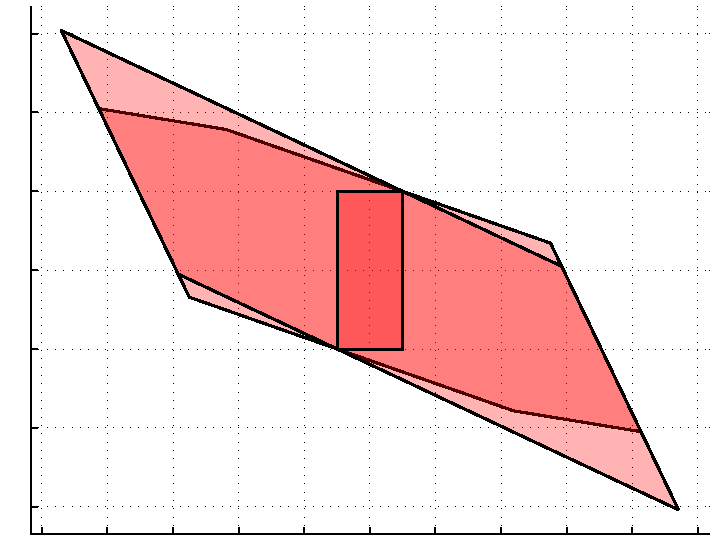
\includegraphics[width=\columnwidth]{twoDimensional}
\caption{The extremal mRPI sets $\mathcal Z^\infty\vert_{({\bf{0}},\theta_{min})}$ and $\mathcal Z^\infty
\vert_{({\bf{0}},\theta_{\max})}$ containing the unit box.}
\label{fig:two:dim:example}
\end{figure}
\begin{figure}
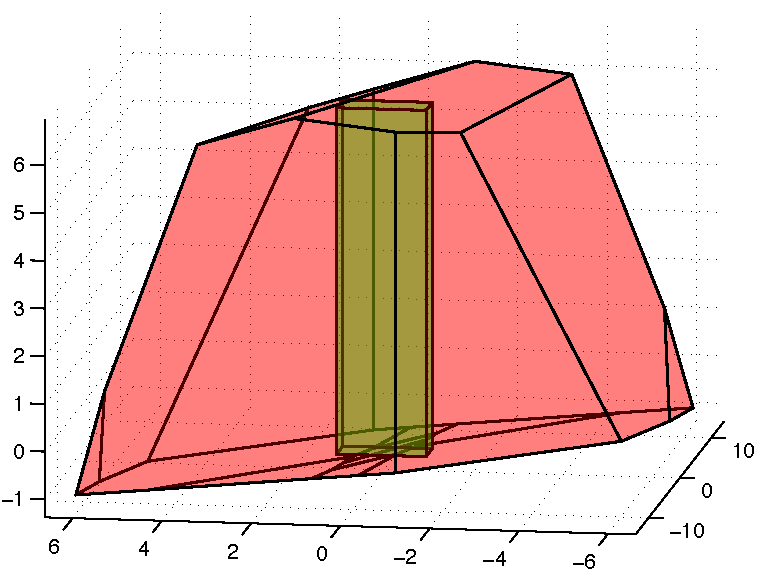
\includegraphics[width=\columnwidth]{threeDimensional}
\caption{The parametrised mRPI set for $\alpha={\bf{0}}$. Containing the unit box in the 
interior between $\theta_{\min}$ and $\theta_{\max}$.}
\label{fig:three:dim:example}
\end{figure}
%
%
%
\section{Conclusions}\label{sec:conclusions}
%
In this paper we discussed extensions to existing computational methods to determine mRPI sets
for linear systems subject to additive disturbance in two cases. The case of state dependent case
which can be applied to determine approximations to mRPI sets for linearised nonlinear systems as was shown
for the example of a levitating ball system. We also introduced the computation of mRPI sets using 
scaling parameters which allows various system analyses using uniform scaling for the disturbance sets
and non-uniform scaling for the input constraints. The effectiveness of state dependent disturbance
sets was demonstrated by comparing the two mRPI methods.
\bibliographystyle{IEEEtran}
\bibliography{IEEEabrv,MyLib}
%
\end{document}